\PassOptionsToPackage{unicode=true}{hyperref} % options for packages loaded elsewhere
\PassOptionsToPackage{hyphens}{url}
\PassOptionsToPackage{dvipsnames,svgnames*,x11names*}{xcolor}
%
\documentclass[]{article}
\usepackage{lmodern}
\usepackage{amssymb,amsmath}
\usepackage{ifxetex,ifluatex}
\usepackage{fixltx2e} % provides \textsubscript
\ifnum 0\ifxetex 1\fi\ifluatex 1\fi=0 % if pdftex
  \usepackage[T1]{fontenc}
  \usepackage[utf8]{inputenc}
  \usepackage{textcomp} % provides euro and other symbols
\else % if luatex or xelatex
  \usepackage{unicode-math}
  \defaultfontfeatures{Ligatures=TeX,Scale=MatchLowercase}
\fi
% use upquote if available, for straight quotes in verbatim environments
\IfFileExists{upquote.sty}{\usepackage{upquote}}{}
% use microtype if available
\IfFileExists{microtype.sty}{%
\usepackage[]{microtype}
\UseMicrotypeSet[protrusion]{basicmath} % disable protrusion for tt fonts
}{}
\IfFileExists{parskip.sty}{%
\usepackage{parskip}
}{% else
\setlength{\parindent}{0pt}
\setlength{\parskip}{6pt plus 2pt minus 1pt}
}
\usepackage{xcolor}
\usepackage{hyperref}
\hypersetup{
            pdftitle={Module 10: Recommended Exercises},
            pdfauthor={Thiago G. Martins, Martina Hall, Stefanie Muff, Department of Mathematical Sciences, NTNU},
            colorlinks=true,
            linkcolor=Maroon,
            filecolor=Maroon,
            citecolor=Blue,
            urlcolor=blue,
            breaklinks=true}
\urlstyle{same}  % don't use monospace font for urls
\usepackage[margin=1in]{geometry}
\usepackage{color}
\usepackage{fancyvrb}
\newcommand{\VerbBar}{|}
\newcommand{\VERB}{\Verb[commandchars=\\\{\}]}
\DefineVerbatimEnvironment{Highlighting}{Verbatim}{commandchars=\\\{\}}
% Add ',fontsize=\small' for more characters per line
\usepackage{framed}
\definecolor{shadecolor}{RGB}{248,248,248}
\newenvironment{Shaded}{\begin{snugshade}}{\end{snugshade}}
\newcommand{\AlertTok}[1]{\textcolor[rgb]{0.94,0.16,0.16}{#1}}
\newcommand{\AnnotationTok}[1]{\textcolor[rgb]{0.56,0.35,0.01}{\textbf{\textit{#1}}}}
\newcommand{\AttributeTok}[1]{\textcolor[rgb]{0.77,0.63,0.00}{#1}}
\newcommand{\BaseNTok}[1]{\textcolor[rgb]{0.00,0.00,0.81}{#1}}
\newcommand{\BuiltInTok}[1]{#1}
\newcommand{\CharTok}[1]{\textcolor[rgb]{0.31,0.60,0.02}{#1}}
\newcommand{\CommentTok}[1]{\textcolor[rgb]{0.56,0.35,0.01}{\textit{#1}}}
\newcommand{\CommentVarTok}[1]{\textcolor[rgb]{0.56,0.35,0.01}{\textbf{\textit{#1}}}}
\newcommand{\ConstantTok}[1]{\textcolor[rgb]{0.00,0.00,0.00}{#1}}
\newcommand{\ControlFlowTok}[1]{\textcolor[rgb]{0.13,0.29,0.53}{\textbf{#1}}}
\newcommand{\DataTypeTok}[1]{\textcolor[rgb]{0.13,0.29,0.53}{#1}}
\newcommand{\DecValTok}[1]{\textcolor[rgb]{0.00,0.00,0.81}{#1}}
\newcommand{\DocumentationTok}[1]{\textcolor[rgb]{0.56,0.35,0.01}{\textbf{\textit{#1}}}}
\newcommand{\ErrorTok}[1]{\textcolor[rgb]{0.64,0.00,0.00}{\textbf{#1}}}
\newcommand{\ExtensionTok}[1]{#1}
\newcommand{\FloatTok}[1]{\textcolor[rgb]{0.00,0.00,0.81}{#1}}
\newcommand{\FunctionTok}[1]{\textcolor[rgb]{0.00,0.00,0.00}{#1}}
\newcommand{\ImportTok}[1]{#1}
\newcommand{\InformationTok}[1]{\textcolor[rgb]{0.56,0.35,0.01}{\textbf{\textit{#1}}}}
\newcommand{\KeywordTok}[1]{\textcolor[rgb]{0.13,0.29,0.53}{\textbf{#1}}}
\newcommand{\NormalTok}[1]{#1}
\newcommand{\OperatorTok}[1]{\textcolor[rgb]{0.81,0.36,0.00}{\textbf{#1}}}
\newcommand{\OtherTok}[1]{\textcolor[rgb]{0.56,0.35,0.01}{#1}}
\newcommand{\PreprocessorTok}[1]{\textcolor[rgb]{0.56,0.35,0.01}{\textit{#1}}}
\newcommand{\RegionMarkerTok}[1]{#1}
\newcommand{\SpecialCharTok}[1]{\textcolor[rgb]{0.00,0.00,0.00}{#1}}
\newcommand{\SpecialStringTok}[1]{\textcolor[rgb]{0.31,0.60,0.02}{#1}}
\newcommand{\StringTok}[1]{\textcolor[rgb]{0.31,0.60,0.02}{#1}}
\newcommand{\VariableTok}[1]{\textcolor[rgb]{0.00,0.00,0.00}{#1}}
\newcommand{\VerbatimStringTok}[1]{\textcolor[rgb]{0.31,0.60,0.02}{#1}}
\newcommand{\WarningTok}[1]{\textcolor[rgb]{0.56,0.35,0.01}{\textbf{\textit{#1}}}}
\usepackage{graphicx,grffile}
\makeatletter
\def\maxwidth{\ifdim\Gin@nat@width>\linewidth\linewidth\else\Gin@nat@width\fi}
\def\maxheight{\ifdim\Gin@nat@height>\textheight\textheight\else\Gin@nat@height\fi}
\makeatother
% Scale images if necessary, so that they will not overflow the page
% margins by default, and it is still possible to overwrite the defaults
% using explicit options in \includegraphics[width, height, ...]{}
\setkeys{Gin}{width=\maxwidth,height=\maxheight,keepaspectratio}
\setlength{\emergencystretch}{3em}  % prevent overfull lines
\providecommand{\tightlist}{%
  \setlength{\itemsep}{0pt}\setlength{\parskip}{0pt}}
\setcounter{secnumdepth}{0}
% Redefines (sub)paragraphs to behave more like sections
\ifx\paragraph\undefined\else
\let\oldparagraph\paragraph
\renewcommand{\paragraph}[1]{\oldparagraph{#1}\mbox{}}
\fi
\ifx\subparagraph\undefined\else
\let\oldsubparagraph\subparagraph
\renewcommand{\subparagraph}[1]{\oldsubparagraph{#1}\mbox{}}
\fi

% set default figure placement to htbp
\makeatletter
\def\fps@figure{htbp}
\makeatother

\usepackage{etoolbox}
\makeatletter
\providecommand{\subtitle}[1]{% add subtitle to \maketitle
  \apptocmd{\@title}{\par {\large #1 \par}}{}{}
}
\makeatother

\title{Module 10: Recommended Exercises}
\providecommand{\subtitle}[1]{}
\subtitle{TMA4268 Statistical Learning V2020}
\author{Thiago G. Martins, Martina Hall, Stefanie Muff, Department of
Mathematical Sciences, NTNU}
\date{March 14, 2020}

\begin{document}
\maketitle

\hypertarget{pca-on-new-york-times-stories}{%
\section{PCA on New York Times
stories}\label{pca-on-new-york-times-stories}}

This exercise is based on the New York Time stories example (code and
data) on the \href{http://www.stat.cmu.edu/~cshalizi/490/10/}{lecture}
of Brian Junker and Cosma Shalizi about Principal components and factor
analysis.

\hypertarget{data-exploration}{%
\subsection{Data Exploration}\label{data-exploration}}

New stories were randomly selected from the
\href{https://catalog.ldc.upenn.edu/LDC2008T19}{New York Times Annotated
Corpus}. There are 57 stories about art and 45 about music on the
dataset available.

The \texttt{nyt\_data} is a dataset containing these 102 stories, which
represent the 102 observations. The first column contains class labels
of the stories (art and music) and, and the other stories contain the
counts of each word in a given story (weight by the inverse document
frequency and normalized by vector length).

The New York Times stories dataset are contained in the file
\texttt{pca-exampes.rdata}, which you can load from google drive
(\url{https://drive.google.com/open?id=1vaK9GDvMw4Hsuv0T1jHeq9ZyrqLhJ6MR})
and store in the directory of your Rmd file. The pca-examples.rdata can
be loaded with the following code.

\begin{Shaded}
\begin{Highlighting}[]
\KeywordTok{load}\NormalTok{(}\StringTok{"pca-examples.rdata"}\NormalTok{)}

\CommentTok{# We will work with nyt.frame}
\NormalTok{nyt_data =}\StringTok{ }\NormalTok{nyt.frame}
\end{Highlighting}
\end{Shaded}

\begin{Shaded}
\begin{Highlighting}[]
\KeywordTok{str}\NormalTok{(nyt_data)}
\KeywordTok{summary}\NormalTok{(nyt_data}\OperatorTok{$}\NormalTok{class.labels)}
\end{Highlighting}
\end{Shaded}

Let's check some word samples:

\begin{Shaded}
\begin{Highlighting}[]
\KeywordTok{colnames}\NormalTok{(nyt_data)[}\KeywordTok{sample}\NormalTok{(}\KeywordTok{ncol}\NormalTok{(nyt_data), }\DecValTok{30}\NormalTok{)]}
\end{Highlighting}
\end{Shaded}

\begin{verbatim}
##  [1] "penchant"  "brought"   "structure" "willing"   "yielding" 
##  [6] "bare"      "school"    "halls"     "challenge" "step"     
## [11] "largest"   "lovers"    "intense"   "borders"   "mall"     
## [16] "classic"   "conducted" "mirrors"   "hole"      "location" 
## [21] "desperate" "published" "head"      "paints"    "another"  
## [26] "starts"    "familiar"  "window"    "thats"     "broker"
\end{verbatim}

Let's check some values in the dataset. We have many zeroes, as most
words do not appear in most stories.

\begin{Shaded}
\begin{Highlighting}[]
\KeywordTok{signif}\NormalTok{(nyt_data[}\KeywordTok{sample}\NormalTok{(}\KeywordTok{nrow}\NormalTok{(nyt_data), }\DecValTok{5}\NormalTok{), }\KeywordTok{sample}\NormalTok{(}\KeywordTok{ncol}\NormalTok{(nyt_data), }\DecValTok{10}\NormalTok{)], }\DecValTok{3}\NormalTok{)}
\end{Highlighting}
\end{Shaded}

\begin{verbatim}
##    jacket patch tapes   want   ford failed condemn intentional confined
## 24      0     0     0 0.0000 0.0000 0.0000       0           0        0
## 2       0     0     0 0.0275 0.0704 0.0000       0           0        0
## 85      0     0     0 0.0482 0.0000 0.0000       0           0        0
## 59      0     0     0 0.0000 0.0000 0.0000       0           0        0
## 76      0     0     0 0.0000 0.0000 0.0215       0           0        0
##    destroyed
## 24         0
## 2          0
## 85         0
## 59         0
## 76         0
\end{verbatim}

\hypertarget{recommended-exercise-1}{%
\section{Recommended exercise 1}\label{recommended-exercise-1}}

\begin{itemize}
\tightlist
\item
  For the New York Times stories (\texttt{nyt\_data}) dataset:

  \begin{itemize}
  \tightlist
  \item
    Create a biplot and explain the type of information that you can
    extract from the plot.
  \item
    Create plots for the proportion of variance explained (PVE) and
    cumulative PVE. Describe what type of information you can extract
    from the plots.
  \end{itemize}
\end{itemize}

\hypertarget{recommended-exercise-2}{%
\section{Recommended exercise 2}\label{recommended-exercise-2}}

Show that the algorithm below is guaranteed to decrease the value of the
objective

\[\underset{C_1, \ldots, C_k}{\text{minimize}}\left\{\sum_{k=1}^{K} \frac{1}{|C_k|} \sum_{i, i' \in C_k} \sum_{j=1}^{p}(x_{ij} - x_{i'j})^2 \right\}\]

at each step.

\center

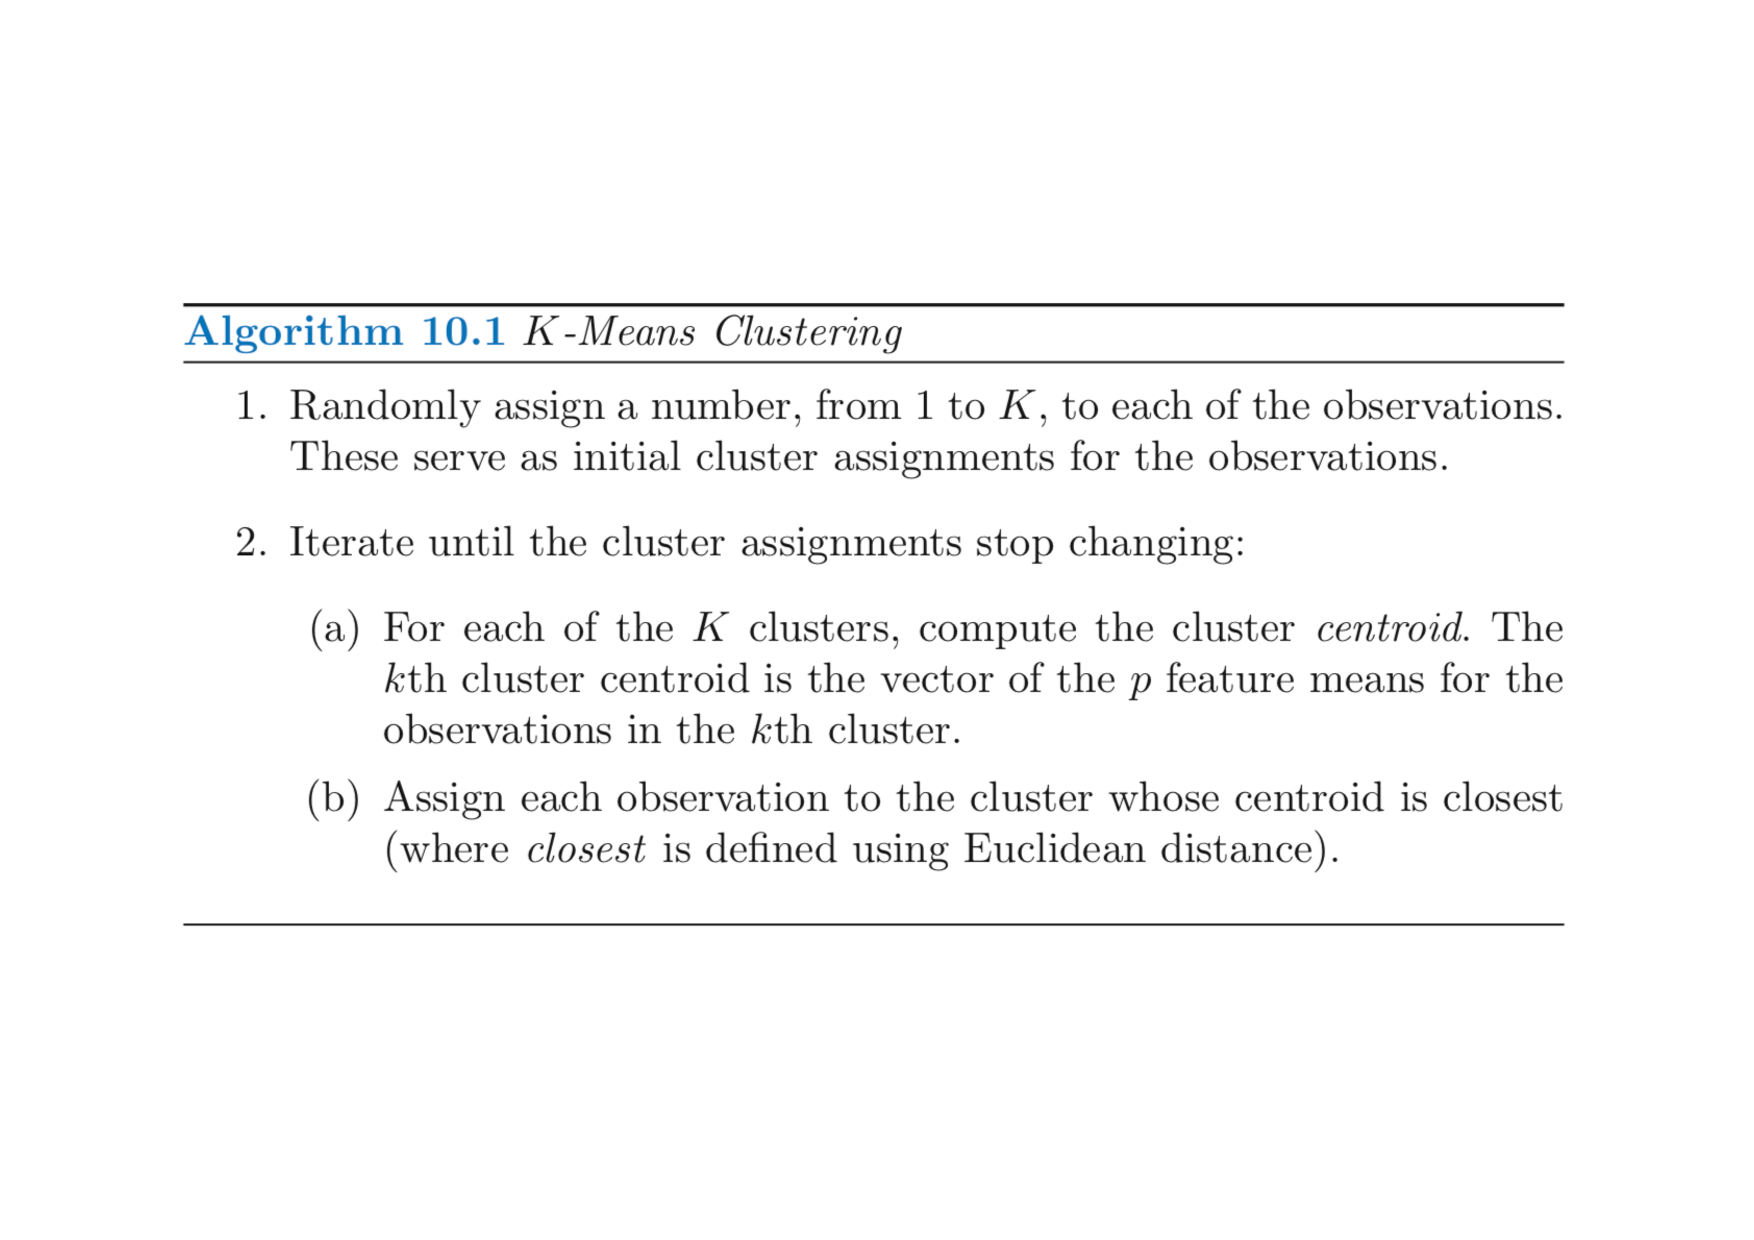
\includegraphics[width=0.8\textwidth,height=\textheight]{kmeans_algo.pdf}

\flushleft

\hypertarget{recommended-exercise-3}{%
\section{Recommended exercise 3}\label{recommended-exercise-3}}

Perform \(k\)-means clustering in the New York Times stories dataset.

\hypertarget{recommended-exercise-4}{%
\section{Recommended exercise 4}\label{recommended-exercise-4}}

Perform hierarchical clustering in the New York Times stories dataset.

\end{document}
